\documentclass{jsarticle}
\usepackage[margin = .7in]{geometry}
\usepackage[dvipdfmx]{graphicx}
\usepackage{listings}
\usepackage{amsmath}
\usepackage{bm}
\usepackage{ascmac}
\lstset{%
  language={python},
  basicstyle={\small},%
  identifierstyle={\small},%
  commentstyle={\small\itshape},%
  keywordstyle={\small\bfseries},%
  ndkeywordstyle={\small},%
  stringstyle={\small\ttfamily},
  frame={tb},
  breaklines=true,
  columns=[l]{fullflexible},%
  numbers=left,%
  xrightmargin=0zw,%
  xleftmargin=3zw,%
  numberstyle={\scriptsize},%
  stepnumber=1,
  numbersep=1zw,%
  lineskip=-0.5ex%
}

\begin{document}
\title{卒論テーマ候補 :ゆびすま}
\author{池上 慧}
\maketitle

\section{ゲームの概要}
\subsection{ゆびすまとは}
「ゆびすま」とは2人以上で行われるゲームである。ここでは2人で行われるケースを想定する。プレイヤーは「攻め」と「守り」の役目を交互に行う。プレイヤーは毎回好きな本数の親指を上げる。「攻め」のプレイヤーは今回上がる親指の本数を予想し、その予想した数をコールしながら、自分でも好きな本数だけ親指を上げる。「守り」のプレイヤーも掛け声と同時に親指を好きな本数だけあげる。「攻め」がコールした数と実際にあげられた親指の総数が等しかったなら「攻め」の勝ちであり、そうでなければ「引き分け」である。引き分けたら役割を交代してどちらかが勝つまで続けるものとする。本来であれば勝てば腕を一本減らすことができ、先に二回勝利した方の勝ちというルールであるが、ここでは最初の2本vs2本の状況のみを想定する。

\subsection{ゲームの構造}
このゲームで勝敗を決するのは攻め手が決定する「宣言」と「指」との差である。この差で攻め手の行動を分類することができる。すなわち相手の上げる指の数が0本の時勝利する行動の組である$\left\{ (0,0), (1,1), (2,2)\right\}$をset1とし、相手の指の数が1本の時に勝利する行動の組である$\left\{ (1,0), (2,1), (3,2)\right\}$をset2、相手の指の数が2本の時に勝利する行動の組である$\left\{ (2,0), (3,1), (4,2)\right\}$をset3とする。これを用いてゲームの利得表は以下のように与えられる。
\begin{figure}[h]
    \centering
    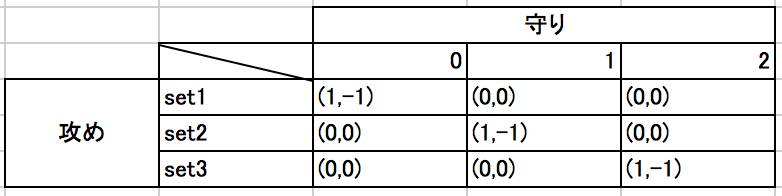
\includegraphics[width=10cm]{pmat.png}
    \caption{利得表}
\end{figure}

これは2人対称ゼロサムゲームとなる。守り手が$\left\{ 0,1,2\right\}$をそれぞれ取る確率を$(q,r,s)$で表記し、攻め手が取るsetに対しての混合戦略、すなわちset1, set2, set3をとる確率を$(x,y,z)$で表記する。この時の混合戦略ナッシュ均衡は以下のようである。これをモデル1と呼ぶ。
\begin{itembox}[l]{ゆびすまゲームのナッシュ均衡}
    \begin{align}
    	\begin{cases}
		(q, r, s) = (\frac{1}{3}, \frac{1}{3}, \frac{1}{3})\\
		(x, y, z) = (\frac{1}{3}, \frac{1}{3}, \frac{1}{3})
	\end{cases}
    \end{align}
\end{itembox}

つまり攻め手も守り手も自身の行動に等しく確率を割り振るのが最適反応を構成している。この時攻め手の本来の行動である$9$個の「宣言」と「指」のペアに対しても等しく$\frac{1}{9}$ずつ確率が振られている。また攻め手の勝利確率は$\frac{1}{3}$である。

\section{研究の目的意識}
しかし上記のように全ての戦略に等しく確率を割り振る戦略が実際のプレイでは取られていない可能性が高い。$[a,b]$で宣言$a$ゆびの数$b$の攻め手の行動を表すことにすると、経験的には$[2,1]$のようなある種中途半端な戦略が$[0,0]$や$[4,2]$のような極端な戦略よりも取られやすい傾向があるようように思える。実際、地域によっては利得構造は変えずに$[0,0]$と$[4,2]$に対して特別な名称を与え、他の行動とは別物として扱われているようである。

まず既存の限定合理性のモデル化によって上記の現象が説明できないかを考える。2人完備情報ゲームに適用可能な限定合理生のモデルとして代表的なものには、均衡を扱う概念としてOsborn and Rubinshtein (1998)で提案されたS(k) EquilibriumやMcKelvey and Palfrey (1995)で提案されたquantal response equilibriumがある。しかし、先に挙げたこのゲームの利得表を見ればわかる通りゆびすまは対称なゲームである。このような単純な構造を持つゲームにおいて均衡下で特定の行動が選ばれがちになるような均衡概念は既存のモデル考えにくい。実際、上記のS(k) equilibriumでは均等に行動するのが均衡下での行動であり、QREにおいても通常用いられるoptimization errorの分布を用いると均等に行動するのが均衡として得られてしまう。

そこで、プレイヤーが自身の戦略や相手の戦略について正しい認知を持てていない、つまり限定合理性というよりも根本的にゲームのルールを把握できていないことにナッシュ均衡がプレイされない原因があるのではないかという仮説を立てる。ここでは、「相手の指を一本ずつ別の主体が動かしているものだと見る」と「自身の行動についてどの組み合わせが無差別かを分かっていない」の二つの原因があると想定し、各誤認が発生している時に攻め手がどのような行動をとるかをモデルから導き、データよりそれぞれの誤認の有無を検証する。

また、一つ目にあげた「相手の指を一本ずつ別の主体が動かしているものだと見る」という誤認はそうとわかっても直せないタイプの誤認であるように思える。つまり、ゆびすまをプレイする前に研究者から「相手の指を別々のものとして見る傾向がある」と指摘されても、適切な修正を施して行動できる攻め手は少ないように思える。一方で、二つ目に挙げた「自身の行動についてどの組み合わせが無差別かを分かっていない」については、「自分の宣言数と指の数の差だけが勝敗を消している」というゲームの構造を理解する手助けをするだけで攻め手は行動を適切に修正することができるように思える。このように、認知の歪みには言われて直せるものと言われても直せないものが存在するということを実験を通して明らかにする。

\section{誤認の帰結}
以下、「相手の指を一本ずつ別の主体が動かしているものだと見る」という誤認を誤認1と、「自身の行動についてどの組み合わせが無差別かを分かっていない」という誤認を誤認2と呼称する。
\subsection{誤認1のみ}
相手の指が上がる確率を$p$とし、どちらの指についても同じ戦略をとるとする。攻め手については先と同様に混合戦略を$(x, y, z)$で表記する。この時このゲームの混合戦略ナッシュ均衡は以下のように求められる。
\begin{itembox}[l]{誤認1のみの時の混合戦略ナッシュ均衡}
\begin{align*}
    	&\begin{cases}
		p = \frac{1}{3}\\
		(x, y, z) = (\frac{1}{3}, \frac{2}{3}, 0)
	\end{cases}\\[10pt]
	&\begin{cases}
		p = \frac{1}{2}\\
		(x, y, z) = (0, 1, 0)
	\end{cases}\\[10pt]
	&\begin{cases}
		p = \frac{2}{3}\\
		(x, y, z) = (0, \frac{2}{3}, \frac{1}{3})
	\end{cases}
\end{align*}
\end{itembox}
このうち安定な均衡は一番上と一番下の二つである。従って、誤認1のみ発生している時は以下の二つの均衡のどちらかをプレイすることになる。これをモデル2と呼ぶ。ただし、これは攻め手のとる行動についてのみ成り立つことであり、守り手は実際にはこの$p$にしたがって行動をとるわけではないことに注意が必要である。
\begin{itembox}[l]{誤認1のみ発生している時の行動}
\begin{align}
    	&\begin{cases}
		p = \frac{1}{3}\\
		(x, y, z) = (\frac{1}{3}, \frac{2}{3}, 0)
	\end{cases}\\[10pt]
	&\begin{cases}
		p = \frac{2}{3}\\
		(x, y, z) = (0, \frac{2}{3}, \frac{1}{3})
	\end{cases}
\end{align}
\end{itembox}
この時、set内の各行動については選択する基準を持っていないため、無差別に選択すると仮定するのが妥当である。つまりsetについては無差別ではないが、set内の行動については無差別である。また、上記二つの行動がそれぞれ確率$(w, 1-w)$でプレイされているとする。守り手はナッシュ均衡に従い指を均等な確率であげるとすると、攻め手の勝利確率は$\frac{1}{3}$である。

\subsection{誤認2のみ}
ここでは攻め手が自身の宣言する数(以降「宣言数」と呼称)と自身のあげる指の数(以降「指」と呼称)とについて、それらを組み合わせた実際の行動に確率を割り振るのではなく、宣言数と指について別々に行動の確率を割り振ることでゲームをプレイする状況を考える。これは混合戦略というよりもbehavioral strategyなので、behavioral strategyの均衡を求める。
\begin{figure}[h]
    \centering
    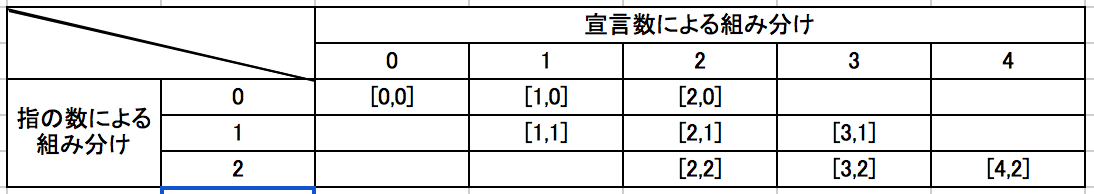
\includegraphics[width=10cm]{class2.png}
    \caption{組み分け}
\end{figure}

上の表を使って考える。宣言数$(0,1,2,3,4)$に対しては対称性より$(p_0, p_1, p_2, p_1, p_0)$の確率を割り振る。表からわかるように、指$(0,1,2)$に対しては宣言数との組み合わせによって勝利条件を決して満たさない組が存在するので、指の数に単純に確率を割り振るだけでは適切な戦略を構成できない。そこで、宣言数が$1, 3$の時に指$1$をあげる確率を$a$、宣言数が$2$の時に指$1$をあげる確率を$b$と表記することにする。また、相手が指$0,2$をあげる確率を$r$と表記する。これを用いてbehavioral strategyの均衡は以下のように求められる。これをモデル3と呼ぶ。

\begin{itembox}[l]{誤認2のみが発生している時の行動}
\begin{align}
	\begin{cases}
    	&p_0 = \frac{1}{3},\ (p_1, p_2) \in \left\{ (p_1, p_2) \mid 2p_1 + p_2 = \frac{1}{3}, p_1 \geq 0, p_2 \geq 0\right\}\\[10pt]
	&(a.b) = (0,1)\\[10pt]
	&r = 0
	\end{cases}
\end{align}
\end{itembox}
この時、setごとの確率は$\frac{1}{3}$であるが、set内の各行動が選ばれる確率は均等ではなくなっていることがわかる。つまりsetについては無差別だが、set内の行動については無差別ではない。これより、守り手がナッシュ均衡に従っているとすれば、攻め手の勝利確率は$\frac{1}{3}$である。

\subsection{誤認1と誤認2}
誤認1と誤認2が同時に発生するケースを考える。具体的には上記の表記を用いて、この時のbehavioral strategyの均衡は以下のようになる。これをモデル4と呼ぶ。
\begin{itembox}[l]{誤認1と誤認2が同時に発生している時の行動}
\begin{align}
	\begin{cases}
    	&0 \leq p_0 \leq \frac{1}{3}, \ (p_1, p_2) \in \left\{ (p_1, p_2) \mid \frac{1}{3} \leq 2p_1 + p_2 \leq 1, p_1 \geq 0, p_2 \geq 0\right\}\\[10pt]
	&0 \leq a, b \leq 1\\[10pt]
	&p = \frac{3\pm \sqrt{3}}{6}
	\end{cases}
\end{align}
\end{itembox}
この時、setについても無差別でなく、set内の行動についても無差別でない行動をとる個人を表現することができる。ここで攻め手の勝利確率は$\frac{1}{3}$である。

\section{実験の枠組みとモデルの評価}
以下の3種類の実験を行う。
\begin{description}
	\item[実験1] 何も説明せずゆびすまをプレイしてもらう
	\item[実験2] 誤認1について説明したのちにゆびすまをプレイしてもらう
	\item[実験3] 誤認2について説明したのちにゆびすまをプレイしてもらう
\end{description}
誤認1は説明によっても治すことができず、誤認2は説明によって治すことができるという仮説が正しければ、実験1ではモデル4、実験2でもモデル4、実験3ではモデル2がそれぞれプレイされるはずである。

そのためにまず、実験1においてモデル4がプレイされていることを確かめる。このために、モデル1から4までを実験1のデータでフィットを比べ、モデル4が最も高い説明力を持っていることを確認する。次に、実験2においてモデル3とモデル4とを比べ、モデル4が高い説明力を持つことを確認する。最後に実験3においてモデル2とモデル4とを比べ、モデル2が高い説明力を持つことを確認する。

\end{document}





























